\chapter{Regilaul: Estonia's {\it runosong} tradition}
\index{Runsong and the Kalevala}@\emph{Runosong and the Kalevala}



\begin{figure}[htbp]
\begin{center}
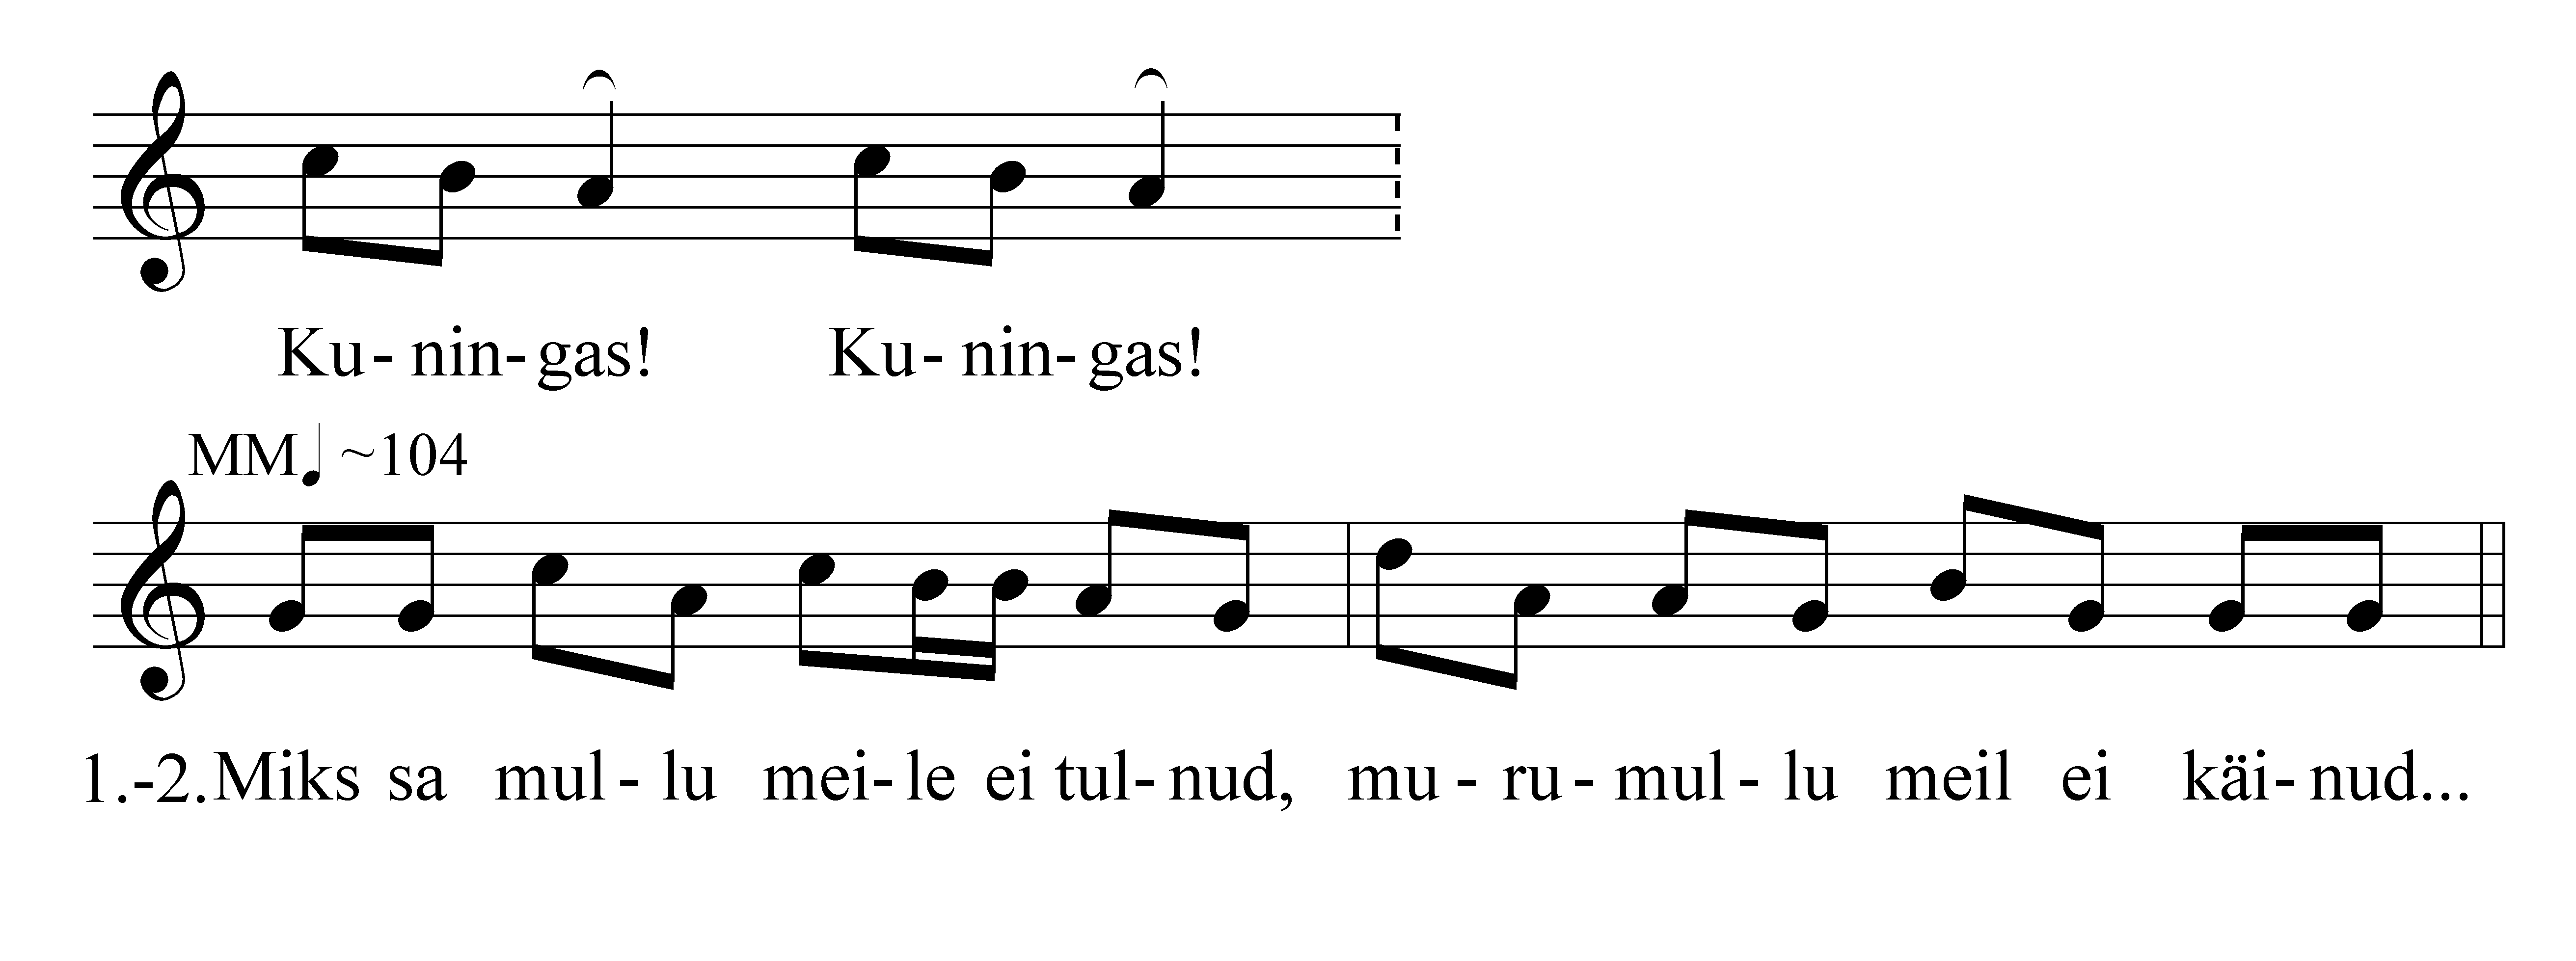
\includegraphics[width=300pt]{figures/094.png}
\caption{music notation of ``The King Game" as performed by Liisa Kümmel}
\label{The King Game}
\end{center}
\end{figure}

\section{The Runic Song Tradition} 


A given {\it regilaul} verse line contains eight beats, generally evenly divided into a single measure so that each of the eight syllables corresponds with one eighth note. The ictus position of a song's line is thus determinable by counting every other beat as ictus, starting with the first.

The first song festival in Estonia held in \cite{ruutelTRADITIONALMUSICESTONIA2004}. 


One runic invariant is that the tonal center is placed on ``the both syntactically stable 


dominating pitch value of the most stable syntactical positions of a given melody's typological group


the syllable-note is the basic unit of the melody-line. Thus syllables take up the space of the note in their position of the melody as prescribed. 


Melodic accents coincide with the stressed syllables, the pitch resolves as the phrase resulves. Said to be a musical abstraction of the natural prosodic intonation of the 8 syllable (spoken) runoverse. 
\cite{ruutelResultsComputerizedComparative1999} 

%
%\section{The singing giant: a common folklore epic} 
%Estonian, Finnish, Karelian, Ingrian runic songs
%
%whether it be Finnish, Estonian, Karelian, Votic, Ingrian and to same extent even Livonian an Veps)
%
%
%the singable song \cite{tormisKalevalaEstonianPerspective1985}
%
%
% ancient epic tale shared by many members of the Finno-Ugric language family
% 
% The common folklore of Finno Ugric language family: Kalavala in Finland, Kalevipoeg (Kalev's son) in Estonia. Kalev is a giant. His companion is a hedgehog.  
% many stories involve a character seeking incantations (song lyrics) to acquire some skill
% 
 
 \cite{tormisProblemsThatRegilaul2007}
\section{regilaul in prosodic contexts}



\cite{lehistePhoneticsMetrics1992}








 
 
\section{Previous Studies with regilaul}

\begin{figure}[htbp]
\begin{center}
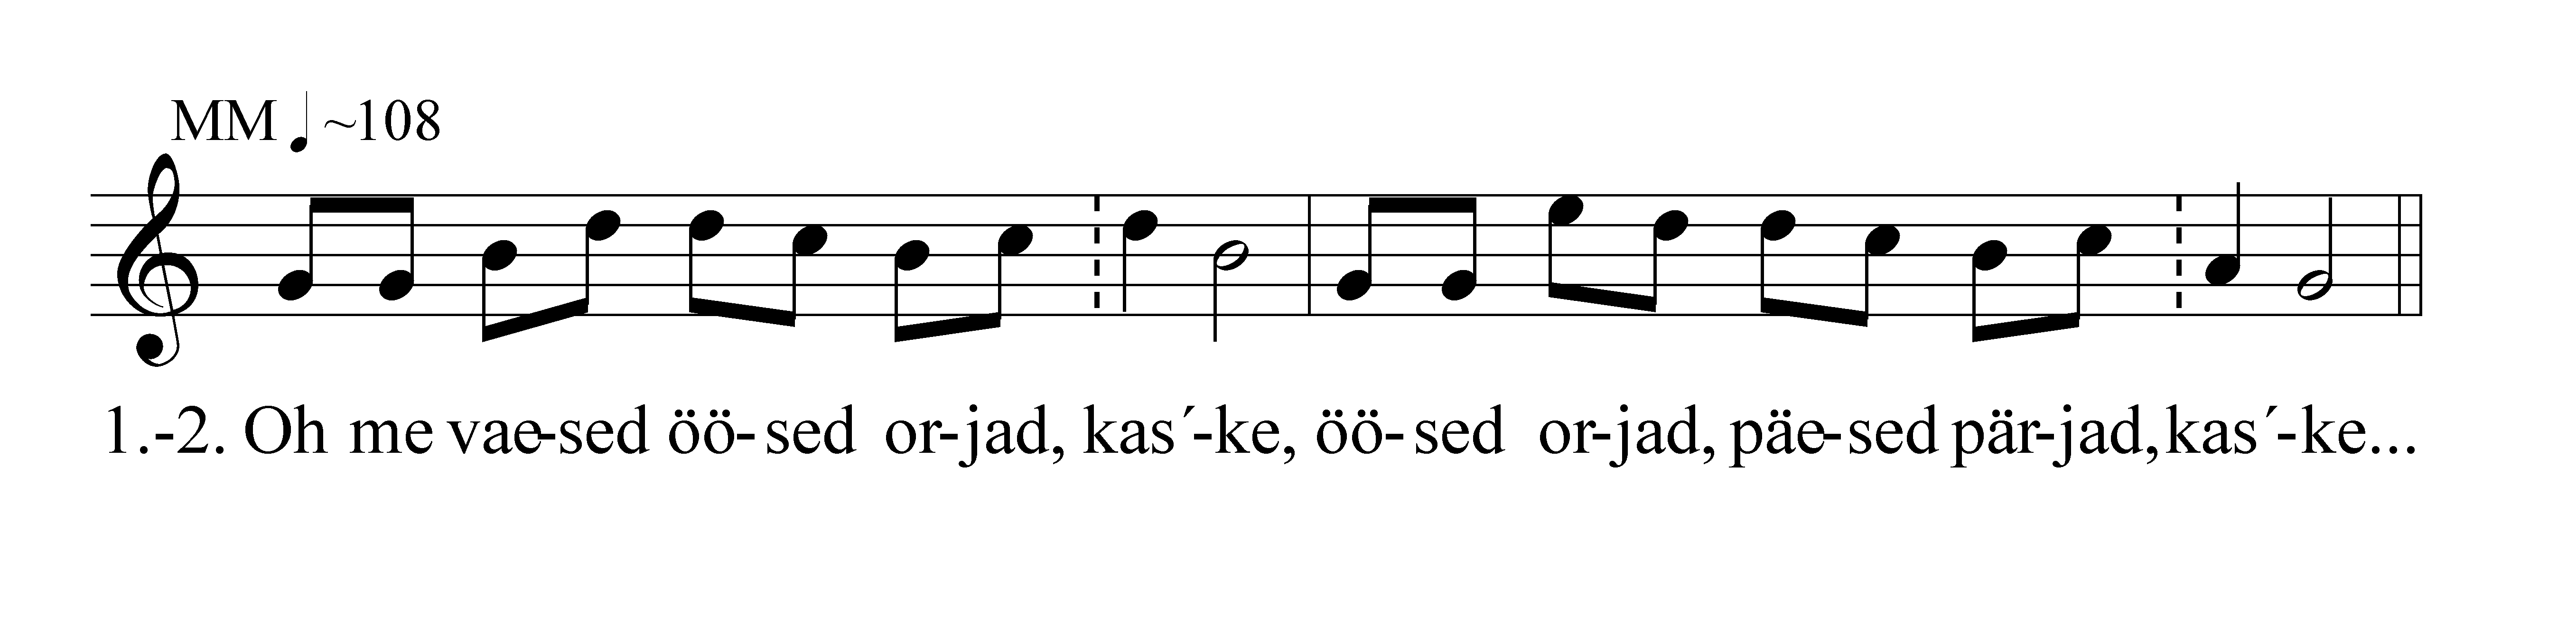
\includegraphics[width=300pt]{figures/069.png}
\caption{default}
\label{default}
\end{center}
\end{figure}

\cite{rossStudyTimingEstonian1989,rossLostProsodicOppositions1994,rossTradeoffQuantityStress1996,sargDoesMelodicAccent2006, sargMelodicAccentEstonian2007,orasMusicalManifestationsTextual2011}
